\subsection{Теории типов}

Изначально, в $\lambda$-исчислении не вводилось никаких правил типизации, однако в дальнейшем появилось множество типизированных вариаций. Барендрегтом в~\cite{barendregt1993lambda} описан так называемый $\lambda$-куб, который наглядно классифицирует восемь различных систем типизации лямбда-исчисления.

\begin{figure}[H]
  \centering
  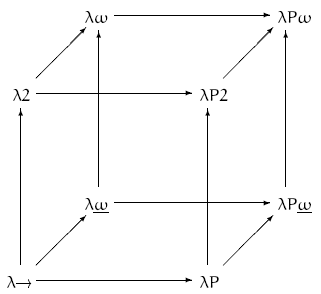
\includegraphics[width=0.5\textwidth]{img/Lambda_cube.png}
  \caption{Лямбда-куб\protect\footnotemark}
\end{figure}

\footnotetext{Изображение взято с сайта \url{https://en.wikipedia.org/wiki/Lambda_cube}, автор -- Денис Москвин}

База куба -- просто типизированное $\lambda$-исчисление($\lambda{\to}$), в котором термы могут зависеть только от термов. Три оси соответствуют расширениям, комбинации которых позволяют получить остальные системы типов:

\begin{enumerate}
  \item Термы, которые зависят от типов -- система $\lambda2$ или \textbf{System F}
  \item Типы, которые зависят от типов -- система $\lambda \underline{\omega}$(операторы над типами)
  \item Типы, которые зависят от термов -- система $\lambda P$(зависимые типы)
\end{enumerate}
